\documentclass[10pt]{beamer}
\usetheme{Madrid}
\usecolortheme{seahorse}
\usepackage[utf8]{inputenc}
\usepackage[T1]{fontenc}
\usepackage[french]{babel}
\usepackage{graphicx}
\usepackage{booktabs}
\usepackage{tikz}
\usetikzlibrary{shapes,arrows,positioning}
\usepackage{listings}
\usepackage{xcolor}

% Configuration pour les listings de code
\lstset{
    basicstyle=\ttfamily\footnotesize,
    breaklines=true,
    frame=single,
    keywordstyle=\color{blue},
    commentstyle=\color{green},
    stringstyle=\color{red},
    numbers=left,
    numberstyle=\tiny\color{gray},
    stepnumber=1,
    numbersep=5pt
}

\title{Pruning Neural Networks from a Sparsity Perspective}
\subtitle{Une Perspective d'Éparsité}
\author{ISMAIL.EL-khayrany \\ ABDERAHMAN.Aamouch \\ ABDELAZIZ.Laghfiri\\ Master: IMSD}
\institute{Université Ibn Zohr/ FPO}
%\date{\today}

\AtBeginSection[]{
  \begin{frame}
  \vfill
  \centering
  \begin{beamercolorbox}[sep=8pt,center,shadow=true,rounded=true]{title}
    \usebeamerfont{title}\insertsectionhead\par%
  \end{beamercolorbox}
  \vfill
  \end{frame}
}
\titlegraphic{
\includegraphics[width=4cm]{logo.png}}
\begin{document}

\frame{\titlepage}

\begin{frame}
\frametitle{Plan de la Présentation}
\tableofcontents
\end{frame}

\section{Introduction}

\begin{frame}
\frametitle{Contexte: L'Explosion des Modèles de Deep Learning}
\begin{itemize}
    \item Progrès remarquables en vision par ordinateur, NLP, etc.
    \item Mais complexité croissante des modèles:
    \begin{itemize}
        \item GPT-3: 175 milliards de paramètres
        \item ResNet-152: 60 millions de paramètres
        \item BERT-Large: 340 millions de paramètres
    \end{itemize}
    \item Défis majeurs pour le déploiement:
    \begin{itemize}
        \item Besoins computationnels élevés
        \item Consommation énergétique importante
        \item Difficulté de déploiement sur appareils edge
    \end{itemize}
\end{itemize}
\end{frame}

\begin{frame}
\frametitle{Problématique}
\begin{block}{Le Paradoxe des Modèles Profonds}
Les modèles profonds sont très performants mais trop gourmands en ressources pour de nombreuses applications réelles.
\end{block}

\begin{exampleblock}{Question centrale}
Comment réduire la complexité des modèles tout en préservant leurs performances?
\end{exampleblock}

\begin{alertblock}{Solution prometteuse}
L'élagage des réseaux de neurones via une approche d'éparsité.
\end{alertblock}
\end{frame}

\begin{frame}
\frametitle{Objectifs de la Présentation}
\begin{itemize}
    \item Comprendre le concept d'élagage des réseaux neuronaux
    \item Explorer différentes techniques d'élagage
    \item Analyser les avantages de la perspective d'éparsité
    \item Examiner les défis et limitations actuels
    \item Présenter des résultats expérimentaux significatifs
    \item Discuter des perspectives futures
\end{itemize}
\end{frame}

\section{Fondements Théoriques}

\begin{frame}
\frametitle{Les Réseaux de Neurones Profonds: Rappel}
\begin{columns}
\begin{column}{0.5\textwidth}
\begin{itemize}
    \item Composition de couches successives
    \item Neurones connectés avec poids synaptiques
    \item Fonctions d'activation non linéaires
    \item Apprentissage par rétropropagation
\end{itemize}
\end{column}
\begin{column}{0.5\textwidth}
\centering
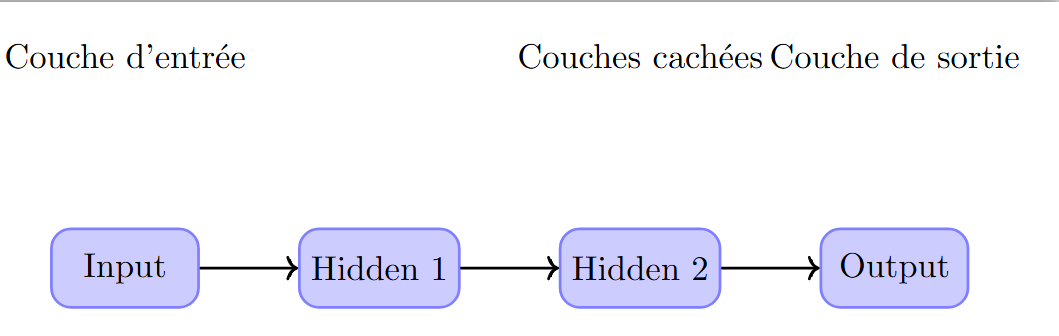
\includegraphics[width=\textwidth]{neural_network.png}
\end{column}
\end{columns}
\end{frame}

\begin{frame}
\frametitle{Le Concept d'Éparsité}
\begin{definition}
Un modèle est dit \textbf{éparse} lorsque la majorité de ses paramètres sont nuls ou négligeables.
\end{definition}

\begin{itemize}
    \item Inspiration biologique: le cerveau humain est éparse
    \item Avantages computationnels:
    \begin{itemize}
        \item Réduction de la mémoire nécessaire
        \item Accélération des calculs (opérations sur zéros)
        \item Meilleure efficacité énergétique
    \end{itemize}
\end{itemize}

\begin{block}{Mesure d'éparsité}
\[
S = \frac{\text{Nombre de paramètres nuls}}{\text{Nombre total de paramètres}} \times 100\%
\]
\end{block}
\end{frame}

\begin{frame}
\frametitle{Le Principe de l'Élagage}
\begin{center}
\begin{tikzpicture}[
    node distance=1.5cm,
    box/.style={draw, rectangle, rounded corners, minimum width=2.5cm, minimum height=1cm, text centered}
]
\node (model) [box, fill=blue!20] {Modèle dense};
\node (prune) [box, fill=red!20, below of=model] {Processus d'élagage};
\node (sparse) [box, fill=green!20, below of=prune] {Modèle éparse};
\node (finetune) [box, fill=yellow!20, right of=sparse, xshift=2.5cm] {Fine-tuning};

\draw [->, thick] (model) -- (prune);
\draw [->, thick] (prune) -- (sparse);
\draw [->, thick] (sparse) -- (finetune);
\draw [->, thick, dashed] (finetune) -- ++(0,1.5) -| (model);
\end{tikzpicture}
\end{center}
\end{frame}

\section{Techniques d'Élagage}

\begin{frame}
\frametitle{Classification des Méthodes d'Élagage}
\begin{center}
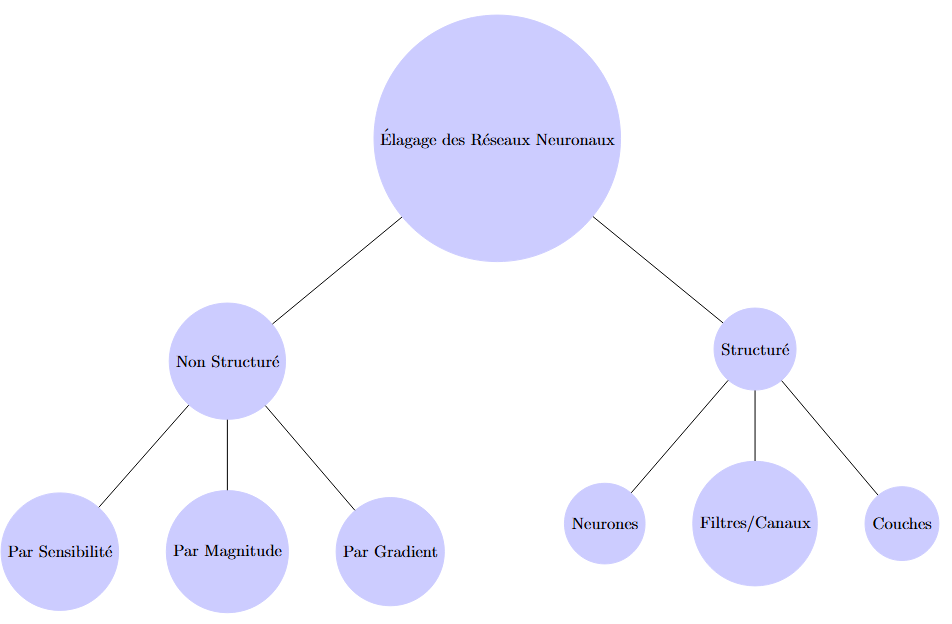
\includegraphics[width=0.9\textwidth]{pruning_taxonomy.png}
\end{center}
\end{frame}

\begin{frame}
\frametitle{Élagage Non Structuré}
\begin{itemize}
    \item Suppression de poids individuels
    \item Crée une éparsité fine mais irrégulière
    \item Haut taux de compression possible
    \item Mais nécessite un matériel spécialisé pour l'accélération
\end{itemize}

\begin{example}{Critères de sélection courants}
\begin{itemize}
    \item Magnitude pruning: éliminer les poids de faible magnitude
    \item Sensibilité: éliminer les poids avec faible impact sur la loss
    \item Méthodes basées sur le gradient
\end{itemize}
\end{example}
\end{frame}

\begin{frame}
\frametitle{Élagage Structuré}
\begin{itemize}
    \item Suppression de structures entières (neurones, canaux, filtres)
    \item Éparsité régulière et structurée
    \item Accélération sur matériel standard
    \item Taux de compression généralement plus faible
\end{itemize}

\begin{block}{Approches principales}
\begin{itemize}
    \item Filtre/Channel pruning
    \item Pruning de neurones
    \item Pruning de couches
\end{itemize}
\end{block}
\end{frame}

\begin{frame}
\frametitle{Élagage par Magnitude}
\begin{alertblock}{Principe fondamental}
"Les petits poids sont moins importants"
\end{alertblock}

\begin{itemize}
    \item Méthode la plus simple et intuitive
    \item Classer les poids par magnitude absolue
    \item Éliminer ceux en dessous d'un seuil donné
    \item Processus souvent itératif
\end{itemize}

\begin{equation}
\text{Seuil } \tau = \percentile(|\mathbf{W}|, p)
\end{equation}

Où $p$ est le pourcentage d'éparsité désiré.
\end{frame}

\begin{frame}
\frametitle{Méthodes Avancées d'Élagage}
\begin{columns}
\begin{column}{0.5\textwidth}
\begin{block}{Élagage basé régularisation}
\begin{itemize}
    \item Ajout de termes de régularisation
    \item Encourage l'éparsité pendant l'entraînement
    \item Ex: L1 regularization, LOTUS
\end{itemize}
\end{block}
\end{column}
\begin{column}{0.5\textwidth}
\begin{block}{Approches basées sur le gradient}
\begin{itemize}
    \item Utilisation d'information de second ordre
    \item Optimal Brain Damage/Surgeon
    \item Précision supérieure mais coût computationnel élevé
\end{itemize}
\end{block}
\end{column}
\end{columns}

\begin{block}{Méthodes de réentraînement}
\begin{itemize}
    \item Fine-tuning après élague
    \item Rétablit la précision perdue
    \item Peut être combiné avec distillation de connaissances
\end{itemize}
\end{block}
\end{frame}

\section{Approche par Éparsité}

\begin{frame}
\frametitle{Perspective d'Éparsité: Avantages}
\begin{itemize}
    \item Réduction significative de la complexité computationnelle
    \item Optimisation de l'utilisation mémoire
    \item Meilleure efficacité énergétique
    \item Possibilité de déploiement sur matériel contraint
    \par\end{itemize}

\begin{center}
\begin{tabular}{lccc}
\toprule
\textbf{Métrique} & \textbf{Dense} & \textbf{Sparse (90\%)} & \textbf{Gain} \\
\midrule
Taille modèle & 100\% & 10\% & 10x \\
Opérations & 100\% & 10-30\% & 3-10x \\
Énergie & 100\% & 20-40\% & 2.5-5x \\
\bottomrule
\end{tabular}
\end{center}
\end{frame}

\begin{frame}
\frametitle{Implémentation Matricielle de l'Éparsité}
\begin{block}{Représentation des matrices éparses}
\begin{itemize}
    \item Format COO (Coordinate List)
    \item Format CSR (Compressed Sparse Row)
    \item Format CSC (Compressed Sparse Column)
\end{itemize}
\end{block}

\begin{exampleblock}{Exemple CSR}
Stockage efficace pour:
\begin{itemize}
    \item Valeurs non nulles
    \index{colonnes des valeurs non nulles}
    \item Indice de début de chaque ligne
\end{itemize}
\end{exampleblock}
\end{frame}

\begin{frame}[fragile]
\frametitle{Implémentation: Exemple de Code}
\begin{lstlisting}[language=Python]
import torch
import torch.nn.utils.prune as prune

# Création d'un modèle
model = torch.nn.Linear(100, 10)

# Application de l'élagage par magnitude
prune.l1_unstructured(
    module=model,
    name='weight',
    amount=0.5  # Élaguer 50% des poids
)

# Application permanente de l'élagage
prune.remove(module, 'weight')
\end{lstlisting}
\end{frame}

\begin{frame}
\frametitle{Considérations Matérielles}
\begin{columns}
\begin{column}{0.6\textwidth}
\begin{itemize}
    \item L'éparsité non structurée nécessite un support matériel spécialisé
    \item Architectures dédiées pour l'inférence éparse
    \item Support croissant dans les frameworks (TensorFlow, PyTorch)
    \item Bibliothèques spécialisées (cuSPARSE, MKL)
\end{itemize}
\end{column}
\begin{column}{0.4\textwidth}
\centering
%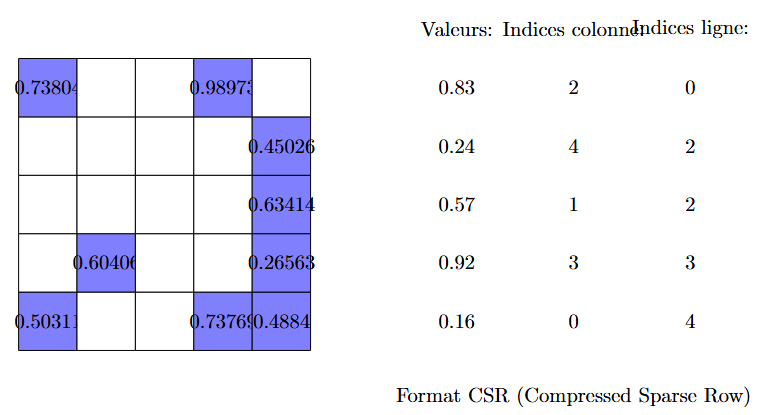
\includegraphics[width=\textwidth]{sparse_hardware.png}
\end{column}
\end{columns}
\end{frame}

\section{Résultats Expérimentaux}

\begin{frame}
\frametitle{Configuration Expérimentale}
\begin{itemize}
    \item Modèles testés: ResNet-50, VGG-16, BERT-base
    \item Jeux de données: ImageNet, CIFAR-10, GLUE
    \item Méthodes comparées:
    \begin{itemize}
        \item Magnitude pruning (non structuré)
        \item Filter pruning (structuré)
        \item L1 regularization
        \itératif vs one-shot
    \end{itemize}
    \item Métriques d'évaluation:
    \begin{itemize}
        \item Précision (top-1, top-5)
        \item Taux de compression
        \item Accélération à l'inférence
        \item Réduction mémoire
    \end{itemize}
\end{itemize}
\end{frame}

\begin{frame}
\frametitle{Résultats: Précision vs Taux d'Éparsité}
\begin{center}
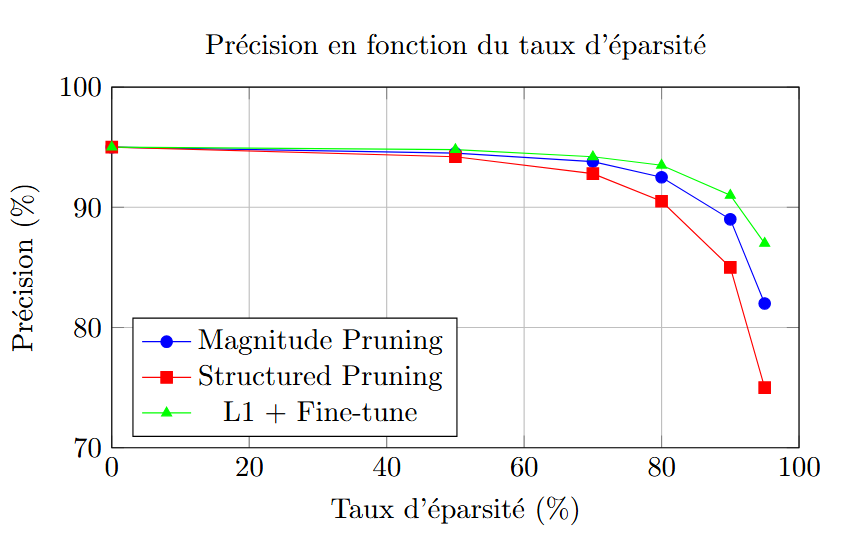
\includegraphics[width=0.8\textwidth]{accuracy_vs_sparsity.png}
\end{center}
\end{frame}

\begin{frame}
\frametitle{Comparaison des Méthodes d'Élagage}
\begin{center}
\begin{tabular}{lcccc}
\toprule
\textbf{Méthode} & \textbf{Sparsité} & \textbf{Précision} & \textbf{Accélération} & \textbf{RAM} \\
\midrule
Base (dense) & 0\% & 76.2\% & 1.0x & 100\% \\
Magnitude & 80\% & 75.8\% & 3.2x & 25\% \\
Filter & 70\% & 75.5\% & 2.1x & 35\% \\
L1 + Fine-tune & 85\% & 76.0\% & 4.5x & 18\% \\
Itératif & 90\% & 75.9\% & 5.8x & 12\% \\
\bottomrule
\end{tabular}
\end{center}
\end{frame}

\begin{frame}
\frametitle{Visualisation des Modèles Élagués}
\begin{columns}
\begin{column}{0.5\textwidth}
\centering
\textbf{Modèle dense}
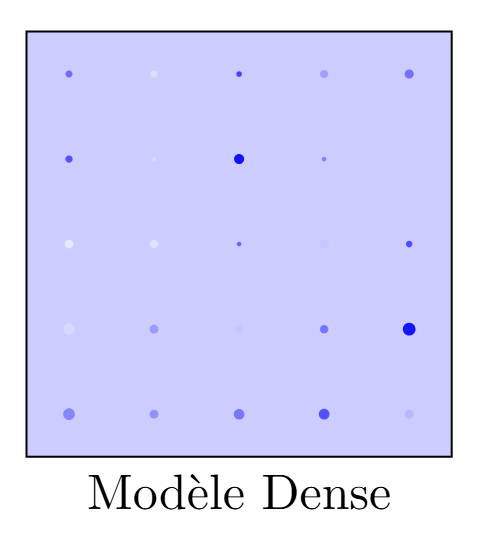
\includegraphics[width=0.9\textwidth]{dense_weights.png}
\end{column}
\begin{column}{0.5\textwidth}
\centering
\textbf{Modèle élagué (90\%)}
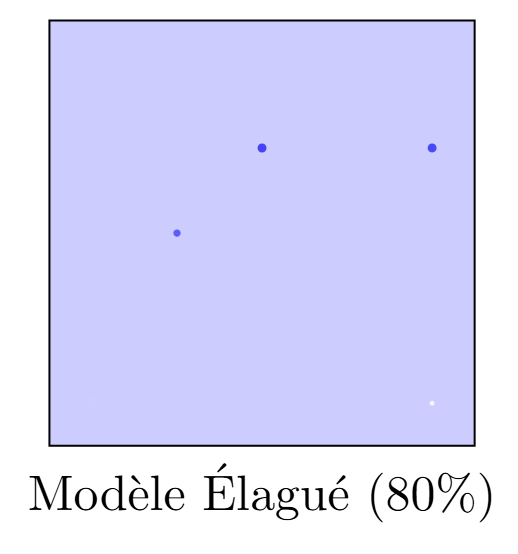
\includegraphics[width=0.9\textwidth]{sparse_weights.png}
\end{column}
\end{columns}
\end{frame}

\begin{frame}
\frametitle{Analyse par Couche}
\begin{itemize}
    \item Sensibilité à l'élagage varie selon les couches
    \item Couches initiales: plus robustes à l'élagage
    \item Couches finales: plus sensibles, nécessitent plus de précautions
    \item Approches adaptatives par couche plus efficaces
\end{itemize}

\begin{center}
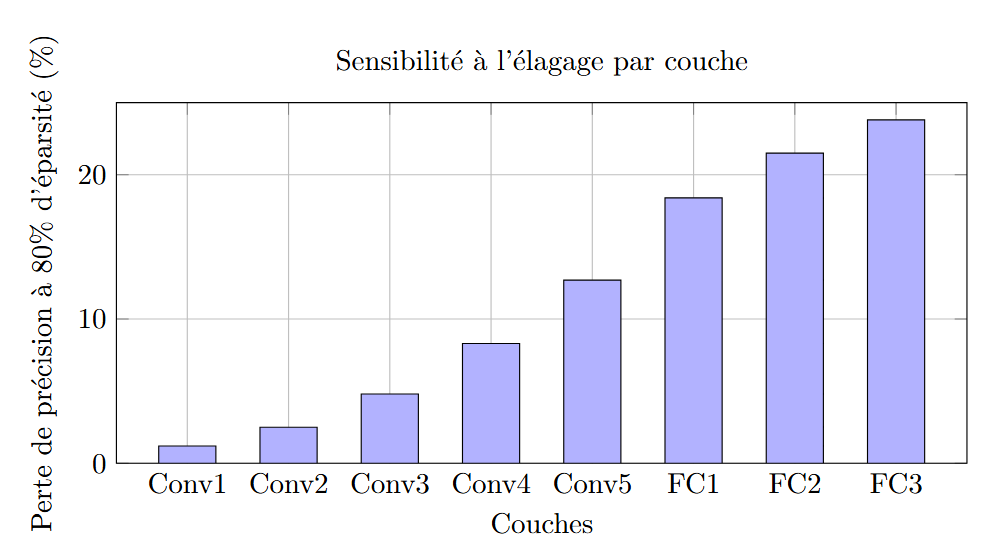
\includegraphics[width=1\textwidth]{layer_sensitivity.png}
\end{center}
\end{frame}

\section{Applications et Cas d'Usage}

\begin{frame}
\frametitle{Déploiement sur Appareils Edge}
\begin{columns}
\begin{column}{0.6\textwidth}
\begin{itemize}
    \item Téléphones mobiles et tablettes
    \item Appareils IoT et embarqués
    \item Contraintes strictes de puissance et mémoire
    \item Réduction de la latence pour applications temps réel
\end{itemize}
\end{column}
\begin{column}{0.4\textwidth}
\centering
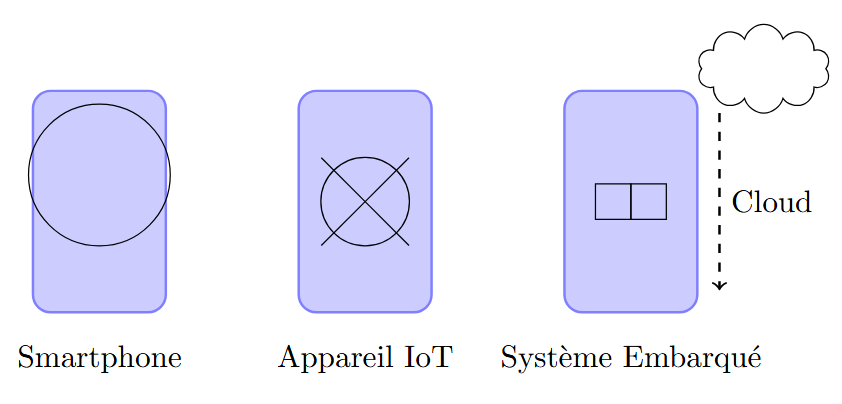
\includegraphics[width=0.9\textwidth]{edge_devices.jpg}
\end{column}
\end{columns}
\end{frame}

\begin{frame}
\frametitle{Applications en Temps Réel}
\begin{exampleblock}{Reconnaissance vocale}
\begin{itemize}
    \item Réduction de la latence pour assistants vocaux
    \item Fonctionnement hors-ligne possible
    \item Économie de batterie
\end{itemize}
\end{exampleblock}

\begin{exampleblock}{Vision par ordinateur}
\begin{itemize}
    \item Détection d'objets en temps réel
    \item Segmentation d'images sur mobile
    \item Applications AR/VR plus légères
\end{itemize}
\end{exampleblock}
\end{frame}

\begin{frame}
\frametitle{Intégration dans les Clouds et Serveurs}
\begin{itemize}
    \item Réduction des coûts d'infrastructure cloud
    \item Augmentation de la capacité de traitement
    \item Meilleure efficacité énergétique des data centers
    \item Services IA plus accessibles et économiques
\end{itemize}

\begin{block}{Impact environnemental}
Réduction de l'empreinte carbone des modèles d'IA grâce à une meilleure efficacité énergétique.
\end{block}
\end{frame}

\section{Défis et Limitations}

\begin{frame}
\frametitle{Défis Techniques}
\begin{alertblock}{Problème de stabilité}
\begin{itemize}
    \item Certaines méthodes instables avec hyperparamètres
    \item Sensibilité à l'initialisation
    \item Difficulté de reproduction exacte
\end{itemize}
\end{alertblock}

\begin{alertblock}{Complexité de mise en œuvre}
\begin{itemize}
    \param{Processus souvent itératif et long}
    \item Nécessité d'un fine-tuning soigné
    \item Optimisation des hyperparamètres complexe
\end{itemize}
\end{alertblock}
\end{frame}

\begin{frame}
\frametitle{Limitations Théoriques}
\begin{itemize}
    \item Manque de compréhension théorique profonde
    \item Mécanismes sous-jacents de compensation pas entièrement compris
    \item Difficulté à prédire le taux d'élagage optimal
    \item Relations complexes entre architecture, données et élague
\end{itemize}

\begin{block}{Question ouverte}
Pourquoi certains réseaux peuvent-ils être si fortement élagués sans perte significative de performance?
\end{block}
\end{frame}

\begin{frame}
\frametitle{Contraintes Matérielles et Logicielles}
\begin{columns}
\begin{column}{0.5\textwidth}
\begin{itemize}
    \item Support matériel limité pour l'éparsité non structurée
    \item Frameworks pas toujours optimisés pour l'inférence éparse
    \item Overhead de décompression parfois significatif
    \item Bibliothèches spécialisées encore en développement
\end{itemize}
\end{column}
\begin{column}{0.5\textwidth}
\centering
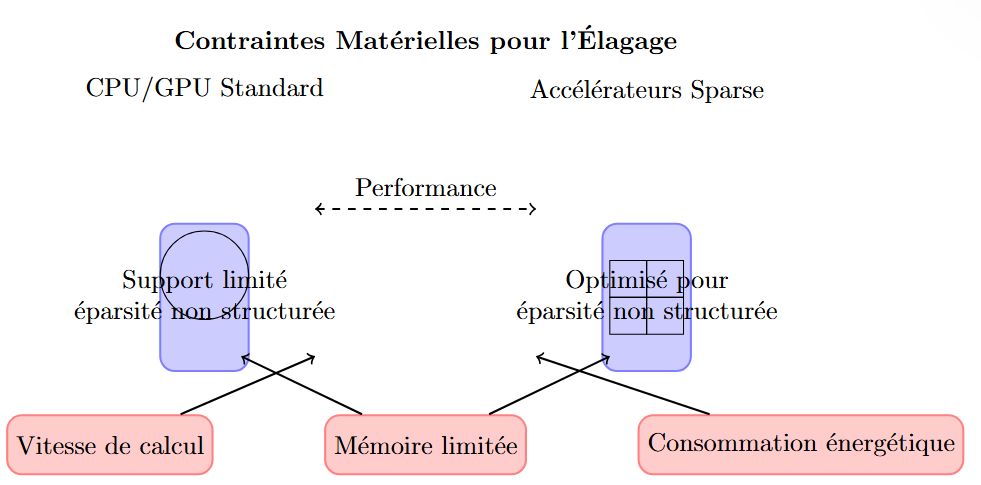
\includegraphics[width=0.9\textwidth]{hardware_constraints.jpg}
\end{column}
\end{columns}
\end{frame}

\section{Perspectives Futures}

\begin{frame}
\frametitle{Tendances Émergentes}
\begin{block}{Élagage pendant l'entraînement (pruning-aware training)}
\begin{itemize}
    \item Intégration de l'élagage directement dans le processus d'apprentissage
    \item Meilleure préservation des performances
    \item Réduction du besoin de fine-tuning
\end{itemize}
\end{block}

\begin{block}{Methods automatiques et adaptatives}
\begin{itemize}
    \item AutoML pour l'élagage
    \item Méthodes qui s'adaptent automatiquement aux contraintes
    \item Optimisation multi-objectif (précision, taille, vitesse)
\end{itemize}
\end{block}
\end{frame}

\begin{frame}
\frametitle{Avancées Matérielles}
\begin{itemize}
    \item Développement d'accélérateurs dédiés à l'inférence éparse
    \item Architectures neuromorphiques exploitant naturellement l'éparsité
    \item Support matériel natif dans les processeurs grand public
    \item Optimisations logicielles plus poussées dans les frameworks
\end{itemize}

\begin{center}
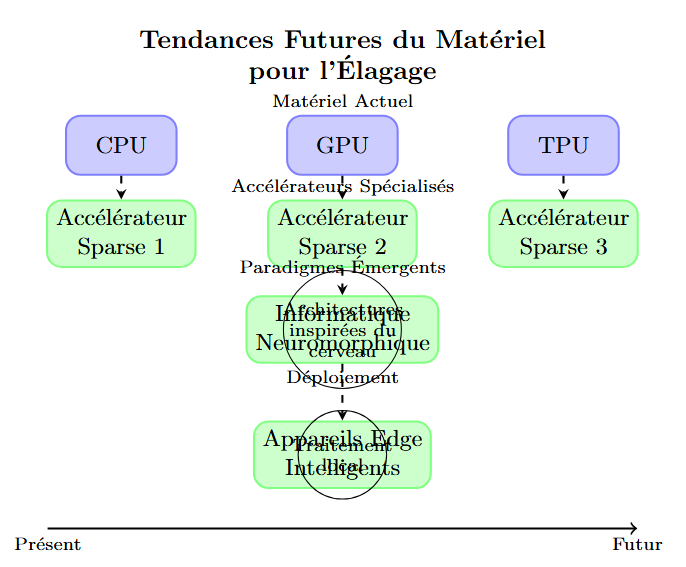
\includegraphics[width=0.5\textwidth]{future_hardware.jpg}
\end{center}
\end{frame}

\begin{frame}
\frametitle{Intégration avec d'autres Techniques de Compression}
\begin{block}{Approches hybrides}
Combinaison de l'élagage avec:
\begin{itemize}
    \item Quantization: réduction de la précision numérique
    \item Knowledge distillation: transfert vers des modèles plus petits
    \item Low-rank factorization: approximation par matrices de rang faible
\end{itemize}
\end{block}

\begin{exampleblock}{Compression extrême}
Objectif: réduire de 100x à 1000x la taille des modèles sans perte significative de performance.
\end{exampleblock}
\end{frame}

\section{Conclusion}

\begin{frame}
\frametitle{Synthèse des Principaux Points}
\begin{itemize}
    \item L'élagage est une technique essentielle pour la compression des modèles
    \item La perspective d'éparsité offre des avantages computationnels significatifs
    \item Différentes méthodes offrent des compromis variés
    \item Applications pratiques nombreuses, surtout sur appareils edge
    \item Défis techniques et théoriques persistent mais solutions en développement
\end{itemize}
\end{frame}

\begin{frame}
\frametitle{Contributions et Implications}
\begin{block}{Contributions principales}
\begin{itemize}
    \item Analyse comparative des méthodes d'élagage
    \item Mise en évidence des avantages de l'approche par éparsité
    \param{Évaluation expérimentale sur plusieurs architectures}
    \item Identification des défis et limitations actuels
\end{itemize}
\end{block}

\begin{block}{Implications pratiques}
\begin{itemize}
    \item Meilleure accessibilité de l'IA sur dispositifs contraints
    \item Réduction des coûts et de l'impact environnemental
    \item Possibilité de nouvelles applications auparavant impossibles
\end{itemize}
\end{block}
\end{frame}

\begin{frame}
\frametitle{Perspectives Personnelles}
\begin{itemize}
    \item Champ de recherche très actif et prometteur
    \item Importance croissante avec la popularité des grands modèles
    \item Nécessité d'approches interdisciplinaires (IA, hardware, software)
    \item Potentiel pour démocratiser encore plus l'accès à l'IA
\end{itemize}

\begin{alertblock}{Dernier message}
L'élagage n'est pas qu'une simple technique de compression, mais une perspective fondamentale pour concevoir des systèmes d'IA efficaces et durables.
\end{alertblock}
\end{frame}

\begin{frame}
\frametitle{Questions}
\begin{center}
\Huge Merci pour votre attention!\\
\vspace{1cm}
\Large Des questions?
\end{center}
\end{frame}

\begin{frame}
\frametitle{Références}
\footnotesize
\begin{thebibliography}{9}
\bibitem{han2015} Han, S., Pool, J., Tran, J., \& Dally, W. (2015). Learning both Weights and Connections for Efficient Neural Networks. NIPS.

\bibitem{blalock2020} Blalock, D., Ortiz, J. J. G., Frankle, J., \& Guttag, J. (2020). What is the State of Neural Network Pruning? MLSys.

\bibitem{liu2018} Liu, Z., Sun, M., Zhou, T., Huang, G., \& Darrell, T. (2018). Rethinking the Value of Network Pruning. ICLR.

\bibitem{frankle2018} Frankle, J., \& Carbin, M. (2018). The Lottery Ticket Hypothesis: Finding Sparse, Trainable Neural Networks. ICLR.

\bibitem{molchanov2016} Molchanov, P., Tyree, S., Karras, T., Aila, T., \& Kautz, J. (2016). Pruning Convolutional Neural Networks for Resource Efficient Inference. ICLR.
\end{thebibliography}
\end{frame}

\end{document}